\chapter{Явления переноса в наноструктурах в поперечном электрическом поле с учетом рассеяния на шероховатой поверхности} \label{chapt4}

\section{Исследования подвижности носителей в квантовых ямах в постоянном поперечном электрическом поле} \label{sect4_1}

Поперечное электрическое поле существенно влияет на явления переноса в наноструктурах. Далее рассмотрим это влияние.
В параболических квантовых ямах (ПКЯ), когда постоянное электрическое поле E направлено вдоль оси пространственного квантования, потенциальная энергия электрона определяется соотношением:
\[
U(z)=\frac{m\omega ^{2} }{2} z^{2} +eEz.
\] 
Следовательно, с ростом напряженности электрического поля минимум $U(z)$ смещается в область отрицательных значений $z$ и опускается на величину $\Delta _{c} ={e^{2} E^{2}  \mathord{\left/{\vphantom{e^{2} E^{2}  (2m\omega ^{2} }}\right.\kern-\nulldelimiterspace} (2m\omega ^{2} } )$. Волновая функция уравнения Шредингера с потенциальной энергией $U(z)$ известна \cite{Sinyavskii1998}, и собственные значения энергии электрона с эффективной массой m в зоне проводимости имеют вид:
\begin{equation} \label{eq:41_10}
E_{n,k_{\bot } } =\frac{\hbar ^{2} k_{\bot } ^{2} }{2m} +E_{n},
\end{equation}
\[
E_{n} =\hbar \omega \left(n+\frac{1}{2} \right)-\Delta _{c} , k_{\bot }^{2} =k_{x}^{2} +k_{y}^{2}.
\] 
$\hbar \omega $ -- энергия размерного квантования, которая простым образом связана с величиной потенциальной энергии $\Delta E_{c} $ на границе ПКЯ с шириной a, $\hbar \omega =\frac{2\hbar }{a} \sqrt{\frac{2\Delta E_{c} }{m} } $, $k_{\bot } $ -- волновой вектор электрона в плоскости низкоразмерной системы.

Из энергетического спектра \eqref{eq:41_10} следует что, минимум зоны проводимости опускается в область запрещенной зоны на величину $\Delta _{c} $. В дальнейшем рассматриваем такие значения напряженности поперечного электрического поля E, при которых параболическая форма потенциальной энергии сохраняется, и в ней остается много размерно-квантованных эквидистантных уровней, т.е. решения уравнения Шредингера с потенциальной энергией U(z) остаются справедливыми \cite{Kanarovskii1995}. Для типичных параметров ПКЯ ($\Delta E_{c} \sim 0.25{\mathrm \; eV}$, $a=10^{3} $Е) $E\le 3\cdot 10^{4} {\mathrm \; V/cm}$. При низких температурах T в нелегированных системах с пониженной размерностью важным является механизм рассеяния носителей на шероховатой поверхности \cite{Sakaki1987,Vurgaftman1999}. В направлениях OX, OY свободного движения носителей заряда ширина ПКЯ изменяется случайным образом, и, следовательно энергия размерного квантования $E_{n} $, определяемая шириной квантовой системы, флуктуирует. Именно по этой причине энергию взаимодействия носителей с шероховатой поверхностью можно записать следующим образом \cite{Sakaki1987}:
\begin{equation} \label{eq:41_20}
W_{n} =\frac{\partial E_{n} }{\partial a} \Delta (x,y)\equiv -\frac{1}{a} \left[E_{n} +2\Delta _{c} \right]\Delta (x,y)=V_{n} \Delta (x,y),
\end{equation}
Здесь $\Delta (x,y)$ -- случайная функция.

Заметим, что энергия взаимодействия для рассматриваемого механизма рассеяния носителей зависит от величины поперечного электрического поля. Для $\delta $-образной флуктуации поверхности
\begin{equation} \label{eq:41_30}
\left\{\Delta (x,y)\Delta (x',y')\right\}=\gamma \delta (x-x')\delta (y-y')\equiv F^{(\delta )} \left(x-x',y-y'\right).
\end{equation} 
В случае гауссовой флуктуации поверхности автокорреляционная функция для различных точек поверхности имеет вид \cite{Sakaki1987}:
\begin{equation} \label{eq:41_40}
\left\{\Delta (x,y)\Delta (x',y')\right\}=\Delta ^{2} {\mathrm exp}\left[-\frac{1}{\Lambda ^{2} } \left((x-x')^{2} +(y-y')^{2} \right)\right]\equiv F^{(G)} \left(x-x',y-y'\right),
\end{equation} 
$\Delta $ -- высота гауссовской флуктуации, $\Lambda $ -- ее длина, $\left\{\right\}$ описывает усреднение по реализации случайного процесса. Заметим, что при низких температурах вид флуктуации поверхности практически не влияет на конечные результаты рассчитываемой наблюдаемой физической величины (например, на электропроводность).

Расчет электропроводности проведем, используя формулу Кубо \cite{Kubo1957a}. В приближении времени релаксации \cite{Khamidullin2002} конечное выражение для электропроводности может быть записано в следующем виде (слабое тянущее электрическое поле направлено вдоль оси OX)
\begin{equation} \label{eq:41_50}
\sigma _{xx} =\frac{e^{2} }{k_{0} TVm^{2} } \sum _{\alpha ,\beta }\left|P_{\alpha \beta }^{\left(x\right)} \right|^{2} \tau _{\alpha } n_{\alpha } \left(1-n_{\beta } \right) ,
\end{equation} 
$\alpha (\beta )$ -- квантовые числа, описывающие состояние электрона, V -- объем основной области размерно-квантованной системы, $P_{\alpha \beta }^{\left(x\right)} $ -- матричный элемент x-ой компоненты оператора импульса на волновых функциях электрона в зоне проводимости, $n_{\alpha } $ -- равновесная функция распределения носителей с энергией $E_{n,k_{\bot } } $, ${1 \mathord{\left/{\vphantom{1 \tau _{\alpha } }}\right.\kern-\nulldelimiterspace} \tau _{\alpha } } $ --квантово-механическая вероятность рассеяния электронов на шероховатой поверхности:
\begin{equation} \label{eq:41_60}
\frac{1}{\tau _{\alpha } } =\frac{2\pi }{\hbar } \sum _{\beta }\tilde{W}_{\alpha \beta } \delta \left(E_{\alpha } -E_{\beta } \right) V_{\alpha } V_{\beta } ,
\end{equation}
где  
\[
\tilde{W}_{\alpha \beta } =\int \Psi _{\alpha }^{*} \left(r\right)\Psi _{\beta }^{*} \left(r_{1} \right)F^{(\delta )} \left(x-x_{1} ,y-y_{1} \right)\Psi _{\alpha } \left(r_{1} \right)\Psi _{\beta } \left(r\right)drdr_{1}  .
\] 
$\Psi _{i} \left(r\right)$ $i=(\alpha ,\beta )$-- волновые функции электрона в ПКЯ в продольном электрическом поле \cite{Sinyavskii1998}.

В случае $\delta $-образной флуктуации поверхности получаем
\begin{equation} \label{eq:41_70}
\frac{1}{\tau _{\alpha } } =\frac{8\gamma \Delta E_{c} }{\hbar a^{4} } \left[\left(n+\frac{1}{2} \right)+N_{c} \right]^{2} , N_{c} =\frac{2\Delta _{c} }{\hbar \omega } .
\end{equation}  
При расчете времени релаксации в случае гауссовской флуктуации поверхности, когда $\frac{\hbar ^{2} }{2m} \Lambda ^{-2} {>>(3 \mathord{\left/{\vphantom{>>(3 2}}\right.\kern-\nulldelimiterspace} 2} )k_{B} T$, что выполняется в широкой области температур, $\frac{1}{\tau _{\alpha } } $ описывается соотношением \eqref{eq:41_70}, в котором нужно $\gamma $ заменить на ($\pi \Delta ^{2} \Lambda ^{2} $). Заметим, что $\tau _{\alpha } $ (для любого типа флуктуации) в точности равно транспортному времени релаксации, используемому при решении кинетического уравнения Больцмана. Как следует из \eqref{eq:41_70}, время релаксации определяется только номером подзоны проводимости. После суммирования по $k_{\bot } $ в \eqref{eq:41_50} электропроводность можно записать в виде:
\begin{equation} \label{eq:41_80}
\sigma _{xx} =\frac{e^{2} }{a\pi \hbar ^{2} \beta _{0} } \sum _{n}\tau _{n} \ln \left(1+e^{-\beta \xi _{n} } \right) , \xi _{n} =E_{n} -\xi ,
\end{equation}
$\xi $ -- химический потенциал.

Для невырожденного электронного газа ($\beta _{0} \xi _{n} >>1$) при низких температурах, когда все носители находятся в нижайшей размерно-квантованной зоне проводимости ($n=0$), подвижность определяется соотношением:
\begin{equation} \label{eq:41_90}
\mu _{xx} =\mu _{xx} (0)\frac{1}{\left(1+2N_{c} \right)^{2} } , \mu _{xx} (0)=\frac{e}{m} \left(\frac{\hbar a^{4} }{2\gamma \Delta E_{c} } \right),
\end{equation} 
где $\mu _{xx} (0)$ -- подвижность в ПКЯ в отсутствии поперечного электрического поля.

Для параметров ПКЯ ($m=0.06m_{0} $) $\hbar \omega =\frac{14.5}{a_{0} } {\mathrm \; eV}$ ($a_{0} $ -- ширина ПКЯ в ангстремах), $N_{c} =1.7\cdot 10^{-18} E_{0}^{2} a_{0}^{3} $ ($E_{0} $ -- измеряется в V/cm). Таким образом, при $a_{0} =10^{3} \AA$, $E_{0} =2.5\cdot 10^{4} {\mathrm \; V/cm}$, $N_{c} =1$ подвижность уменьшается почти на порядок. С ростом E носители тока «прижимаются» к одной из поверхностей квантовой ямы, поэтому их взаимодействие с шероховатой поверхностью увеличивается, что приводит к уменьшению времени релаксации, а следовательно и подвижности.

С ростом температуры процессы рассеяния носителей на длинноволновых акустических колебаниях начинают влиять на величину подвижности. Для случая упругого рассеяния электронов, находящихся на нижайшем уровне зоны проводимости $n=0$ ($\hbar \omega >>k_{B} T$), на акустических фононах при высоких температурах ($N_{q} \approx \frac{k_{B} T}{hvq} >>1$) время релаксации имеет вид:
\begin{equation} \label{eq:41_100}
\frac{1}{\tau _{f} } =\left(\frac{m\omega }{2\pi \hbar } \right)^{\frac{1}{2} } \frac{E_{1}^{2} mk_{B} T}{\hbar ^{3} v^{2} \rho } , 
\end{equation} 
$E_{1} $~--~константа деформационного потенциала, $\rho $ -- плотность исследуемой квантовой системы, $v$~--~скорость звука, $N_{q} $~--~функция распределения равновесных фононов.

Заметим, что $\tau _{f} $ не зависит от волнового вектора электрона и поперечного электрического поля. Электропроводность с учетом рассеяния носителей на шероховатой поверхности ($\tau _{0} $) и на акустических фононах ($\tau _{f} $) определяется соотношением (8), в котором $\frac{1}{\tau _{n} } =\frac{1}{\tau _{0} } +\frac{1}{\tau _{f} } $. Конечное выражение для подвижности принимает вид:
\begin{equation} \label{eq:41_110}
\mu _{xx} =\mu _{xx} (0)\frac{1}{\left(1+2N_{c} \right)^{2} +\Delta } , 
\end{equation} 
\[
\Delta =\left(\frac{m\omega }{2\pi \hbar } \right)^{\frac{1}{2} } \left(\frac{E_{1} }{\hbar \omega } \right)^{2} \frac{4k_{B} Ta^{2} }{\rho v^{2} \gamma }. 
\] 

Для ПКЯ с параметрами ($E_{1} =10{\mathrm \; eV}$,$\rho =4{\mathrm \; }{{\mathrm g} \mathord{\left/{\vphantom{{\mathrm g} {\mathrm cm}^{{\mathrm 3}} }}\right.\kern-\nulldelimiterspace} {\mathrm cm}^{{\mathrm 3}} } $,$v=3\cdot 10^{5} {\mathrm \; }{{\mathrm cm} \mathord{\left/{\vphantom{{\mathrm cm} {\mathrm s}}}\right.\kern-\nulldelimiterspace} {\mathrm s}} $,$\gamma ^{{\tfrac{1}{4}} } =40 \AA$) при $E=2.5\cdot 10^{4} {\mathrm \; V/cm}$. Рассеяние носителей на акустических колебаниях определяет величину подвижности при $T\ge 100{\mathrm \; K}$.

С ростом напряженности поперечного электрического поля минимум зоны проводимости смещается в запрещенную зону на $\Delta _{c} $, а экстремум валентной зоны поднимается на величину $\Delta _{v} ={e^{2} E^{2}  \mathord{\left/{\vphantom{e^{2} E^{2}  (2m_{v} }}\right.\kern-\nulldelimiterspace} (2m_{v} } \omega _{v}^{2} )$ ($\hbar \omega _{v} $ -- шаг размерного квантования валентной зоны). Следовательно, ширина запрещенной зоны E${}_{g}$ в рассматриваемой модели низкоразмерных систем уменьшается на $\Delta _{c} +\Delta _{v} $. Именно это обстоятельство приводит к тому, что с увеличением E однозонное приближение при исследовании явлений переноса может оказаться не достаточным. В этом случае для расчета электропроводности необходимо учитывать нестандартность зоны проводимости \cite{Lax1960,Cohen1961}. Это приводит к тому, что процессы рассеяния электрона на акустических колебаниях становятся зависящими от E. Отметим, что рассмотренное нами влияние поперечного поля E на электропроводность принципиально отличается от эффекта поля в условиях размерного квантования, исследованного в \cite{Sandomirsky1967,Butenko1998}. В этих работах низкоразмерная система (пленка висмута) являются одной из обкладок конденсатора, и ее заряжают, прикладывая поле E, изменяя в ней концентрацию заряда. Именно поэтому при фиксированной толщине КЯ меняется положение уровня Ферми, что приводит к зависимости электропроводности от величины поперечного электрического поля.

\section{Влияние поперечного электрического поля на подвижность в нанопроволоках} \label{sect4_2}

Для квантовых проволок электрическое поле E, направленное перпендикулярно оси наноструктуры, может заметным образом влиять на кинетические явления в размерно-ограниченной системе. В модели потенциала в форме параболоида вращения (такая модель часто применяется при расчетах кинетических коэффициентов в нанопроволоках \cite{Geiler1998,Cros1992} и находит свое математическое подтверждение \cite{Beenakker1991}), в поперечном электрическом поле E энергия электронов с эффективной массой $m_{c} $ в размерно-квантованной зоне c и энергетический спектр дырок с эффективной массой $m_{v} $ в валентной зоне v имеют вид:

\begin{equation} \label{eq:42_10}
\begin{aligned}
E_{\alpha }^{c} =\frac{\hbar ^{2} k_{x}^{2} }{2m_{c} } +E_{nm}^{c} \textbf{ ; } E_{nm}^{c} =\hbar \omega _{c} \left(n+k+1\right)-\Delta _{c} ,\\
E_{\alpha }^{v} =\Delta -\frac{\hbar ^{2} k_{x}^{2} }{2m_{v} } +E_{nm}^{v} \textbf{ ; } E_{nm}^{v} =\hbar \omega _{v} \left(n+k+1\right)-\Delta _{v} . (1)
\end{aligned}
\end{equation}


Здесь $\hbar \omega _{c} $ -- шаг размерного квантования в c зоне, $\hbar \omega _{v} $ -- энергия размерного квантования в валентной зоне, которые простым образом связаны с величиной потенциальной энергии $\Delta E_{i} $ на границе нанопроволоки диаметром a,
\[\hbar \omega _{i} =\frac{2\hbar }{a} \sqrt{\frac{2\Delta E_{i} }{m_{i} } } ,\] 
\[\Delta _{c} =\frac{e^{2} E^{2} }{2m_{c} \omega _{c}^{2} } , \Delta _{v} =\frac{e^{2} E^{2} }{2m_{v} \omega _{v}^{2} } ,\] 
$k_{x} $ -- волновой вектор носителя вдоль оси нанопроволоки.

\begin{figure}[h] 
	\center
	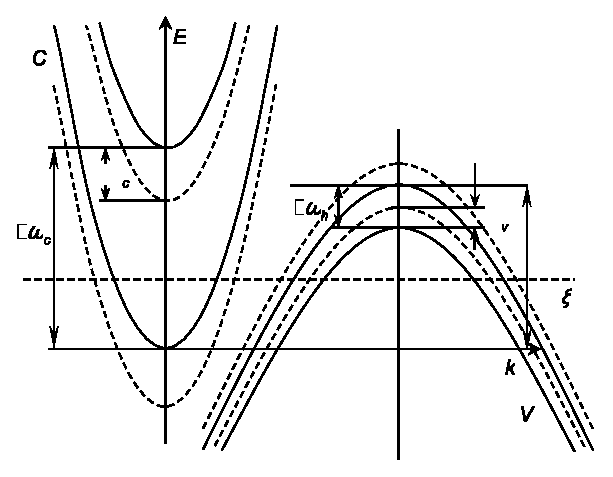
\includegraphics [scale=1] {4_2_1}
	\caption{Схема зонной структуры, рассматриваемой низкоразмерной структуры. Сплошными линиями показаны две нижайшие размерно-квантованные зоны (с-- зоны проводимости, v -- валентные зоны) , пунктирными линиями изображены две нижайшие размерно-квантованные зоны в поперечном электрическом поле; $\xi $ -- химический потенциал.} 
	\label{img:fig_4_2_1} 
\end{figure}

В дальнейшем рассматриваем квантовую проволоку Bi в простой модели, энергетический спектр которой изображен на рис. \ref{img:fig_4_2_1} . Как следует из \eqref{eq:42_10}, с ростом напряженности электрического поля E дно размерно-квантованных c зон опускается на $\Delta _{c} $ в область запрещенных значений энергии, а экстремумы размерно-квантованных v зон поднимаются вверх на величину $\Delta _{v} $.

В квантовых проволоках, как следствие одномерности квантовой системы, на дне размерно-квантованных зон возникают особенности в плотности энергетических состояний. Поэтому, если рассматривать случай вырожденного электронного (дырочного) газа, то с ростом E экстремумы, например размерно-квантованных c зон, опускаясь вниз, пересекают химический потенциал, что может приводить к особенностям электропроводности (подвижности) в исследуемой наноструктуре.

Расчет электропроводности проведем, используя формулу Кубо \cite{Kubo1957a}. В приближении времени релаксации \cite{Khamidullin2002} выражение для электронной электропроводности записывается следующим образом (слабое тянущее электрическое поле направлено вдоль оси нанопроволоки):
\begin{equation} \label{eq:42_20}
\sigma _{xx}^{(e)} =\frac{e^{2} }{k_{0} TVm_{c}^{2} } \sum _{\alpha \beta }\left|\hat{P}_{\alpha \beta }^{(x)} \right|^{2} \tau _{\alpha }^{(e)} n_{\alpha } \left(1-n_{\beta } \right),
\end{equation} 
$\alpha ,\beta $ -- квантовые числа, описывающие состояние электрона, V -- объем основной области размерно-квантованной системы, T -- температура, $k_{0} $ -- постоянная Больцмана, $\hat{P}_{\alpha \beta }^{(x)} $ -- матричный элемент x-ой компоненты оператора импульса на волновых функциях электрона в нанопроволоке, $n_{\alpha } $ -- равновесная функция распределения носителей с энергией $E_{\alpha } $; ${1 \mathord{\left/{\vphantom{1 \tau _{\alpha }^{(e)} }}\right.\kern-\nulldelimiterspace} \tau _{\alpha }^{(e)} } $ -- квантово-механическая вероятность рассеяния в единицу времени.

В дальнейшем исследуем случай рассеяния носителей на шероховатой поверхности, которое оказывается наиболее важным при низких температурах \cite{Sakaki1987,Vurgaftman1999}. В направлении x свободного движения носителей заряда в квантовой проволоке диаметр a меняется случайным образом и, следовательно, энергия размерного квантования $E_{nm}^{(i)} $, определяемая a, флуктуирует. Именно по этой причине энергию взаимодействия носителей с шероховатой поверхностью записывают в виде \cite{Sakaki1987}:
\begin{equation} \label{eq:42_30}
W_{nk}^{(i)} =\frac{\partial E_{nm}^{(i)} }{\partial a} \Delta (x)=-\frac{1}{a} \left[\hbar \omega _{i} \left(n+k+1\right)+2\Delta _{i} \right]\Delta (x)\equiv V_{nk} \Delta (x),  (3)
\end{equation}  
$\Delta (x)$ -- случайная функция.

Как следует из \eqref{eq:42_30}, энергия взаимодействия носителей с шероховатой поверхностью определяется величиной напряженности поперечного электрического поля и с ростом $E$ увеличивается. Последнее обстоятельство приводит, как будет показано ниже, к заметной зависимости подвижности от величины электрического поля.

Для $\delta $-образной флуктуации поверхности автокорреляционная функция для различных точек поверхности нанопроволоки имеет вид:
\begin{equation} \label{eq:42_40}
\left\{\Delta (x)\Delta (x')\right\}=\gamma \delta (x-x'),
\end{equation} 
Обратим внимание, что вид флуктуации ($\delta $-образный или гауссовый \cite{Sakaki1987}) при низких температурах практически не влияет на конечные результаты физической величины (например на подвижность).

Расчет времени релаксации $\tau _{\alpha } $ проводится аналогично \cite{Karapetyan2011}:
\begin{equation} \label{eq:42_50}
\frac{1}{\tau _{\alpha } } =\frac{2m_{c} \omega _{c}^{2} \gamma }{\hbar a^{2} \left|k_{x} \right|} \left(n+k+1+N_{c} \right)^{2} , N_{c} =\frac{2\Delta _{c} }{\hbar \omega _{c} } .
\end{equation} 
Согласно \eqref{eq:42_50} время релаксации зависит от всех квантовых чисел, определяющих состояние носителя, и в точности совпадает с транспортным временем релаксации, используемом при решении кинетического уравнения Больцмана.

Если использовать \eqref{eq:42_20} и \eqref{eq:42_50}, то выражение для подвижности носителей в рассматриваемой модели принимает вид:
\begin{equation} \label{eq:42_60}
\mu =\mu _{0} \frac{\sqrt{\pi } }{2\sum _{nm}F(\eta _{nm}^{c} ) } \sum _{nm}\left\{\frac{\ln \left[\exp \left(\eta _{nm}^{c} \right)+1\right]}{\left(n+m+1+N_{c} \right)^{2} } +\left(\frac{\Delta E_{c} }{\Delta E_{v} } \right)\frac{1}{p} \frac{\ln \left[\exp \left(\eta _{nm}^{v} \right)+1\right]}{\left(n+m+1+N_{v} \right)^{2} } \right\} . 
\end{equation} 
Здесь введены обозначения:
\[
\eta _{nm}^{c} =\frac{1}{k_{0} T} \left[\xi -\hbar \omega _{c} \left(n+m+1\right)+\Delta _{c} \right],\] 
\[\eta _{nm}^{v} =\frac{1}{k_{0} T} \left[-\xi -\hbar \omega _{v} \left(n+m+1\right)+\Delta +\Delta _{v} \right],
\] 
\[
\mu _{0} =\frac{4R^{4} e}{\gamma \Delta E_{c} } \sqrt{\frac{k_{0} T}{2\pi m_{c} } } ; R=\frac{a}{2} ; N_{c} =\frac{2\Delta _{c} }{\hbar \omega _{c} } ; N_{v} =\frac{2\Delta _{v} }{\hbar \omega _{v} } ,
\] 
\[
F(\eta _{nm}^{c} )=\int _{0}^{\infty }\frac{dx}{\exp \left(x^{2} -\eta _{nm}^{c} \right)+1}  ,
\] 
$p$ -- число c зон, участвующих в процессах электропроводности. Химический потенциал $\xi $ находится из условия электронейтральности исследуемой наноструктуры (число электронов в зонах проводимости равно числу дырок в валентной зоне)
\begin{equation} \label{eq:42_70}
p\sqrt{\frac{m_{c} }{m_{v} } } \sum _{n,m}\int _{0}^{\infty }\frac{dx}{\exp \left(x^{2} -\eta _{nm}^{c} \right)+1}   =\sum _{n,m}\int _{0}^{\infty }\frac{dx}{\exp \left(x^{2} -\eta _{nm}^{v} \right)+1}. 
\end{equation} 
Положение химического потенциала при заданных параметрах наносистемы определяется величиной радиуса R квантовой проволоки и величиной напряженности поперечного электрического поля.

Рассмотрим частные случаи, допускающие аналитическое решение уравнения \eqref{eq:42_70}. Пусть электронный (дырочный) газ является невырожденным. Это возможно, если радиус квантовой проволоки такой, что $\Delta <\hbar \omega _{c} +\hbar \omega _{v} $. Как показали экспериментальные исследования \cite{Black2003a} при $R=250 \AA$ в нанопроволоках Bi $\Delta =\hbar \omega _{c} +\hbar \omega _{v} $. Если $m_{c} <<m_{v} $ и носители находятся в нижайших размерно-квантованных зонах (n = m = 0), подвижность можно записать в следующем виде:
\begin{equation} \label{eq:42_80}
\mu =\mu _{0} \frac{1}{\left(1+N_{c} \right)^{2} } .
\end{equation}
Согласно \eqref{eq:42_80} подвижность в рассматриваемом случае с ростом напряженности поперечного электрического поля убывает. Это связано с более сильным взаимодействием носителей с шероховатой поверхностью с увеличением электрического поля. Если электронный газ вырожден и химический потенциал расположен между нижайшей и последующей размерно-квантованной зоной проводимости (аналогично и для размерно-квантованной v зоны), то подвижность описывается следующим соотношением:
\begin{equation} \label{eq:42_90}
\mu =\mu _{0} \frac{\sqrt{2\pi } }{4\left(1+N_{c} \right)^{2} } \left[\frac{1}{k_{0} T} \left(\Delta +\Delta _{A} +\Delta _{v} -\hbar \omega _{v} -\hbar \omega _{A} \right)\right]^{\frac{1}{2} }
\end{equation} 
Как непосредственно следует из \eqref{eq:42_90}, подвижность с ростом E убывает, но слабее, чем в случае невырожденного электронного газа. В общем случае зависимость подвижности от напряженности поперечного электрического поля можно найти только численно.

\noindent \includegraphics*[width=6.19in, height=4.20in, keepaspectratio=false]{image402}

\noindent Рис. 2. Зависимость подвижности (в относительных единицах) от напряженности поперечного электрического поля. $R=330 \AA$

Влияние поперечного электрического поля на подвижность принципиальным образом зависит от радиуса нанопроволоки. При небольших значениях $R$, когда квантовая проволока представляет почти безщелевой полупроводник, с ростом $E$ (при $E=0$ электронный (дырочный) газ невырожден) подвижность сначала уменьшается (см формулу \eqref{eq:42_80}), затем увеличивается, и в дальнейшем описывается осцилляционной кривой (рис. 2). При больших радиусах нанопроволок, когда электронный (дырочный) газ изначально был вырожден, зависимость $\mu $ от $E$ носит явно осциллирующий характер (рис. 3). Такое поведение подвижности в присуствии поперечного электрического поля связано со следующим: с ростом напряженности поперечного электрического поля, дно размерно-квантованных c зон, опускаясь в область запрещенных значений энергии, пересекают химический потенциал, что приводит к увеличению подвижности. Заметим, что для типичных значений параметров нанопроволок Bi ($m_{c} =0.01m_{0} $,$m_{v} =0.1m_{0} $,${\Delta E_{c}  \mathord{\left/{\vphantom{\Delta E_{c}  \Delta E_{v} }}\right.\kern-\nulldelimiterspace} \Delta E_{v} } =1.5$) $N_{v} =5.8N_{c} $, поэтому с ростом $E$ влияние дырок на поведение $\mu $ от $E$ слабее, чем для электронов. Следовательно, осцилляционная зависимость подвижности от $E$ (рис. 3) должна наблюдаться и для полупроводниковых квантовых проволок с вырожденным электронным газом.

\includegraphics*[width=6.33in, height=4.50in, keepaspectratio=false]{image403}

\noindent Рис. 3. Зависимость подвижности (в относительных единицах) от напряженности поперечного электрического поля. $R=990 \AA$



\section{Особенности подвижности в нанопроволоках в поперечных электрическом и магнитном полях} \label{sect4_3}
Теперь рассмотрим одновременное влияние магнитного и электрического полей на явления переноса в квантовых проволоках. В присутствии однородного квантующего магнитного поля энергетический спектр носителей в квантовых проволоках заметным образом меняется. В модели параболического потенциала для нанопроволок радиуса $R$ энергия электрона с учетом анизотропии эффективных масс (магнитное поле H  направлено перпендикулярно оси наноструктуры, электрическое поле E параллельно H) определяется аналогично \cite{Geiler1998}.

\begin{equation} \label{eq:43_10}
	E_{k_x,n,m}=\frac{{\hbar }^2k^2_x}{2m^*_x}+\hbar {\Omega }_y\left(n+\frac{1}{2}\right)+\hbar {\omega }_z\left(m+\frac{1}{2}\right)-{\Delta }_c,   
\end{equation}
\[
m^*_x=m_x{\left(\frac{{\Omega }_y}{{\omega }_y}\right)}^2,\ \ {\Omega }^2_y=\frac{m_x}{m_y}{\left({\omega }^c_x\right)}^2+{\omega }^2_y,\ \ {\omega }^c_x=\frac{eH}{m_xc},\ \ {\omega }_i=\frac{1}{R}{\left[\frac{2\Delta E_c}{m_i}\right]}^{\frac{1}{2}},\ \ {\Delta }_c=\frac{{\left(eER\right)}^2}{4\Delta E_c}
\]
$k_x$ -- волновой вектор электрона вдоль оси квантовой проволоки, $\hbar {\omega }_z,\ \ \hbar {\Omega }_y$ -- энергии размерного квантования, $\Delta E_c$ -- высота потенциальной энергии на границе наноструктуры.

Заметим, что с ростом напряженности электрического поля дно размерно-квантованной зоны проводимости опускается в область запрещенной зоны.

Расчет тензора электропроводности проведем с использованием формулы Кубо
\cite{Kubo1957a} (слабое тянущее электрическое поле направлено вдоль оси нанопроволоки). В приближении времени релаксации \cite{Khamidullin2002} электропроводность записывается следующим образом 

В дальнейшем рассмотрим случай рассеяния заряженных частиц на шероховатой поверхности наносистемы \cite{Sakaki1987},  который является доминирующим при малых радиусах квантовой проволоки и низких температурах. При этом энергию взаимодействия носителей с шероховатой поверхностью записываем в следующем виде \cite{Sakaki1987,Motohisa1992}:
\begin{equation} \label{eq:43_30} 
W_{\alpha }=\frac{\partial E_{\alpha }}{\partial R}\Delta \left(x\right)\equiv V_{\alpha }\Delta \left(x\right) 
\end{equation}
\[
V_{\alpha }=-\frac{1}{R}\left[{\left(\frac{{\omega }_y{\omega }^c_x}{{\Omega }^2_y}\right)}^2\frac{m_y}{m_x}\frac{{\hbar }^2k^2_x}{m_x}+\hbar {\omega }_y\left(\frac{{\omega }_y}{{\Omega }_y}\right)\left(n+\frac{1}{2}\right)+\hbar {\omega }_z\left(m+\frac{1}{2}\right)+2{\Delta }_c\right]
\] 
$\Delta \left(x\right)$ -- случайная функция.

Для $\delta $-образной флуктуации поверхности автокорреляционная функция для различных точек поверхности имеет вид:
\[
\left\{\Delta \left(x\right)\Delta \left(x'\right)\right\}={\gamma }_0\delta \left(x-x'\right),
\] 
а усреднение проводится по реализации случайного процесса.  Как непосредственно следует из \eqref{eq:43_30}, с ростом напряженности поперечного электрического поля E взаимодействие электрона с шероховатой поверхностью увеличивается. Расчет времени релаксации с учетом \eqref{eq:43_30} проводится аналогично \cite{Karapetyan2011}. В результате
\begin{equation} \label{eq:43_40} 
\frac{1}{{\tau }_{\alpha }}={\Gamma }_{\alpha }\frac{1}{\left|k_x\right|},\ {\Gamma }_{\alpha }=\frac{2{\gamma }_0m^*_x}{{\hbar }^3}V^2_{\alpha }.  
\end{equation}
Заметим, что время релаксации \eqref{eq:43_40} в точности равно транспортному времени релаксации, используемому при решении кинетического уравнения Больцмана.

Если учесть, что матричный элемент импульса определяется соотношением\footnote{Недиагональные по осцилляторному квантовом числу матричные элементы при разумных параметрах КП дают незначительный в искомую электропроводность}:
\[
{\hat{P}}^{\left(x\right)}_{\alpha \beta }=\hbar k_x{\left(\frac{{\omega }_y}{{\Omega }_y}\right)}^2{\delta }_{\alpha \beta },
\] 
то выражение для электропроводности \eqref{eq:43_20} с учетом \eqref{eq:43_40} принимает вид \eqref{eq:42_20};

В дальнейшем рассматриваем низкие температуры, когда $\hbar {\omega }_z\gg k_0T$, поэтому зависимостью $V_{\alpha }$ от волнового вектора электрона можно пренебречь. В этом естественном приближении соотношение \eqref{eq:43_50}, после интегрирования по $k_x$, можно записать:
\begin{equation} \label{eq:43_60}
{\sigma }_{xx}=\frac{2e^2\hbar }{{\beta }_0{\pi }^2m^*_x{\gamma }_0}\sum_{nm}{\frac{{ln \left[1+{exp \left({\beta }_0{\xi }_{nm}\right)\ }\right]\ }}{{\left[\hbar {\omega }_y\frac{{\omega }_y}{{\Omega }_y}\left(n+\frac{1}{2}\right)+\hbar {\omega }_z\left(m+\frac{1}{2}\right)+2{\Delta }_c\right]}^2}} 
\end{equation}
\[
{\xi }_{nm}=\xi -\hbar {\Omega }_y\left(n+\frac{1}{2}\right)-\hbar {\omega }_z\left(m+\frac{1}{2}\right)+{\Delta }_c,\ \ \beta =\frac{1}{k_0T}
\]
$\xi $ -- химический потенциал исследуемой наносистемы. Аналогично можно записать ${\sigma }_{xx}$ для дырок в T валентной зоне полуметалла Bi. В этом случае в \eqref{eq:43_60} эффективные массы электронов нужно заменить на соответствующие массы дырок ${\mu }_x,{\mu }_y,{\mu }_z$, а $\xi $  на $-\xi +{\Delta }_0$ (${\Delta }_0$ определяется перекрыванием T валентной зоны и зоны проводимости, ${\Delta }_0\cong 39\ meV$ \cite{Levin2009a}) 

Энергия электронов в валентной зоне определяется соотношением:
\[
E^v_{\alpha }={\Delta }_0-\frac{{\hbar }^2k^2_x}{2{\mu }^*_x}-\hbar {\widetilde{\Omega }}_y\left(n+\frac{1}{2}\right)-\hbar {\widetilde{\omega }}_z\left(m+\frac{1}{2}\right)+{\Delta }_v,
\] 
здесь обозначено
\[
{\mu }^*_x={\mu }_x{\left(\frac{{\widetilde{\Omega }}_y}{{\widetilde{\omega }}_y}\right)}^2,\ {\widetilde{\Omega }}^2_y=\frac{{\mu }_x}{{\mu }_y}{\left({\widetilde{\omega }}^c_x\right)}^2+{\widetilde{\omega }}^2_y,\ \ {\widetilde{\omega }}^c_x=\frac{eH}{{\mu }_xc},\ \ {\widetilde{\omega }}_i=\frac{1}{R}{\left[\frac{2\Delta E_v}{{\mu }_i}\right]}^{\frac{1}{2}},\ \ {\Delta }_v=\frac{{\left(eER\right)}^2}{4\Delta E_v}
\] 
$\hbar {\widetilde{\Omega }}_y, \hbar {\widetilde{\omega }}_z$ -- энергия размерного квантования в валентной зоне, $\Delta E_v$ -- высота потенциальной энергии для дырок на границе квантовой проволоки.

Следовательно, подвижность носителей (электронов и дырок) в нанопроволоке записывается следующим образом:
\begin{multline} \label{eq:43_70} 
\mu =\frac{eR^2{\hbar }^2}{m^*_x{\gamma }_0}\frac{1}{\sqrt{2m^*_x{\beta }_0}\sum_{nm}{F\left({\xi }_{nm}\right)}}\sum_{nm}{\frac{{\ln \left[1+{\exp \left(\beta {\xi }_{nm}\right)\ }\right]\ }}{{\left[\hbar {\omega }_y\frac{{\omega }_y}{{\Omega }_y}\left(n+\frac{1}{2}\right)+\hbar {\omega }_z\left(m+\frac{1}{2}\right)+2{\Delta }_c\right]}^2}}+\\
+\frac{eR^2{\hbar }^2}{{\mu }^*_x{\gamma }_0}\frac{1}{\sqrt{2{\mu }^*_x{\beta }_0}\sum_{nm}{F\left({\widetilde{\xi }}_{nm}\right)}}\sum_{nm}{\frac{{\ln \left[1+{\exp \left(\beta {\widetilde{\xi }}_{nm}\right)\ }\right]\ }}{p{\left[\hbar {\widetilde{\omega }}_y\frac{{\widetilde{\omega }}_y}{{\widetilde{\Omega }}_y}\left(n+\frac{1}{2}\right)+\hbar {\widetilde{\omega }}_z\left(m+\frac{1}{2}\right)+2{\Delta }_v\right]}^2}} 
\end{multline}
\[
F\left({\xi }_{nm}\right)=\int^{\infty }_0{\frac{dx}{{exp \left(x^2-\beta {\xi }_{nm}\right)\ }+1}},
\]
\[
{\widetilde{\xi }}_{nm}=-\xi -\hbar {\widetilde{\Omega }}_y\left(n+\frac{1}{2}\right)-\hbar {\widetilde{\omega }}_z\left(m+\frac{1}{2}\right)+{\Delta }_0+{\Delta }_v
\]
p -- число С зон, участвующих в процессах электропроводности. Если магнитное поле направлено вдоль оси OZ, а постоянное поперечное электрическое поле E перпендикулярно H, то подвижность, как показывают расчеты, тоже описывается соотношением \eqref{eq:43_70}.

Химический потенциал $\xi $ находится из условия электронейтральности исследуемой квантовой проволоки (число электронов в p зонах проводимости равно числу дырок в валентной зоне):
\begin{equation} \label{eq:43_80} 
p{\left(\frac{m^*_x}{{\mu }^*_x}\right)}^{\frac{1}{2}}\sum_{nm}{F\left({\xi }_{nm}\right)}=\sum_{nm}{F\left({\widetilde{\xi }}_{nm}\right)} (8) 
\end{equation}

Из \eqref{eq:43_80} следует что, величина химического потенциала $\xi $ зависит от радиуса нанопроволоки и определяется напряженностью электрического и магнитного полей.

Дальнейшие оценки будем проводить для параметров, близких к полуметалу Bi: $m_x=0.0011m_0$, $m_y=0.26m_0$, $m_z=0.0045m_0$, ${\mu }_x={\mu }_y=0.059m_0$, ${\mu }_z=0.634$ \cite{Levin2009a}, ${\Delta }_c=0.5\ eV$, ${\Delta }_v=0.3\ eV$ ($m_0$ -- масса свободного электрона). При этих параметрах
\[
\hbar {\omega }_y=\frac{4.9}{R_0}\left(eV\right),\ \hbar {\omega }_z=\frac{37.6}{R_0}\left(eV\right),\ \hbar {\widetilde{\omega }}_y=\frac{8}{R_0}\left(eV\right),\ \ \hbar {\widetilde{\omega }}_z=\frac{2.4}{R_0}\left(eV\right)\ ,
\] 
($R_0$ -- радиус нанопроволоки в ангстремах).

\noindent \includegraphics*[width=5.21in, height=4.89in, keepaspectratio=false]{image404}

\noindent Рис. 1. Зависимость подвижности в относительны единицах $\widetilde{{\mathbf \mu }}={{\mathbf \mu }\left(E\right)}/{{\mathbf \mu }\left(0\right)}$ от электрического поля.

На рис. 1 приведены численные расчеты зависимости подвижности (в относительных единицах) от напряженности поперечного электрического поля. Кривые 1,2,3 получены при $\ \delta =0,$ $\delta =0.05$, $\delta =0.1$ соответсвенно $\left(\delta ={\left(\frac{{\omega }^c_x}{{\omega }_y}\right)}^2\right)$. При малых значениях ${\Delta }_c$ электронный газ (при рассмотренных параметрах квантовой проволоки) является невырожденным, поэтому с ростом напряженности поперечного электрического поля уменьшается \cite{Karapetyan2012}. Кривая 1 (подвижность в отсутствии  магнитного поля) описывается тремя максимумами. Такая осцилляционная зависимость подвижности связана с тем, что с ростом $E$ химический потенциал, отсчитанный от дна размерно-квантованной зоны проводимости, поднимается в область больших значений энергии и может «наткнуться» на дно размерно-квантованной C зоны, в которой существуют особенности в плотности энергетических состояний. Первый пик связан с пересечением химического потенциала нижайшего состояния размерно-квантованной C зоны $\left(n=0,m=0\right)$, второй пик возникает из-за пересечения химического потенциала дна первой размерно-квантованной зоны $\left(m=0,n=1\right),$ третий пик -- из-за пересечения химического потенциала второй размерно-квантованной зоной $\left(m=1,n=0\right)$. С ростом напряженности магнитного поля дно размерно-квантованной зоны проводимости поднимается в область больших значений энергии, поэтому пересечение химического потенциала наступает при больших значениях ${\Delta }_c$. Именно по этой причине первый пик кривой 2  сдвинут по отношению первого пика кривой 1 в область больших значений напряженности поперечного электрического поля.

Заметим, что согласно \eqref{eq:43_70} подвижность с ростом напряженности магнитного поля уменьшается. Это связано с тем, что эффективные массы электронов (дырок) в однородном поперечном магнитном поле увеличиваются (в ${\left(\frac{\Omega_y}{\omega_y}\right)}^2$ раз для электронов и в ${\left(\frac{{\widetilde{\Omega }}_y}{{\widetilde{\omega }}_y}\right)}^2$ раз для дырок).

\section{Термоэдс в нанопроволоках Bi в попереченом постоянном электрическом поле}\label{sect4_4}

В квантовых проволоках, как следствие одномерности исследуемой наносистемы, на дне размерно-квантованных зон возникают особенности в плотности энергетических состояний. Именно это обстоятельство приводит, в частности, к особенностям оптических свойств нанопроволок \cite{Black2003a,Black2000,Black2002,Levin2009a}, и заметным образом влияет, как будет показано ниже, на кинетические коэффициенты в нанопроволоках с вырожденным электронным (дырочным) газом. В настоящей диссертационной работе теоретически исследуется термоэдс в квантовых проволоках типа Bi в модели квадратичного потенциала. Такая модель часто применяется при расчетах кинетических коэффициентов в нанопроволоках \cite{Geiler1998,Geiler1999} и находит свое теоретическое обоснование \cite{Beenakker1991}. Если постоянное электрическое поле $E$, направленное вдоль оси размерного квантования наноструктуры при определенных условиях может существенным образом влиять на подвижность \cite{Karapetyan2011}, то представляет интерес исследовать влияние $E$ на термоэдс в низкоразмерных системах.
 
В квантовых проволоках типа Bi с потенциальной энергией для носителей в форме параболоида вращения в постоянном электрическом поле E, направленном перпендикулярно оси исследуемой наноструктуры. В рассматриваемой модели энергия электронов с эффективной массой $m_{c} $ в размерно-квантованной зоне проводимости имеет вид:
\begin{equation} \label{eq:44_10}
\varepsilon _{c} =\frac{\hbar ^{2} k_{x}^{2} }{2m_{c} } +\hbar \omega _{c} \left(n+k+1\right)-\Delta _{c} , \Delta _{c} =\frac{e^{2} E^{2} }{2m_{c} \omega _{c}^{2} } , 
\end{equation} 
здесь $k_{x} $ -- волновой вектор носителя вдоль оси нанопроволоки, $\hbar \omega _{c} $ -- шаг размерного квантования, который простым образом связан с величиной потенциальной энергии $\Delta E_{c} $ на границе наноструктуры с радиусом R:
\[
\hbar \omega _{c} =\frac{\hbar }{R} \sqrt{\frac{2\Delta E_{c} }{m_{c} } } .
\] 

Как непосредственно следует из (1) с ростом напряженности электрического поля дно размерно-квантованной зоны проводимости опускается в запрещенную зону. Именно это обстоятельство приводит к тому, что при учете рассеяния электронов на шероховатой поверхности время релаксации зависит от E, что и приводит к заметному изменению кинетических коэффициентов \cite{Karapetyan2011}. С ростом E носители «прижимаются» к поверхности наноструктуры, т.е. их взаимодействие с шероховатой поверхностью увеличивается, что приводит к уменьшению времени релаксации. Аналогичным образом можно вычислить энергию электронов с эффективной массой $m_{v} $ в размерно-квантованной валентной зоне.
\begin{equation} \label{eq:44_20}
\varepsilon _{v} =\Delta -\frac{\hbar ^{2} k_{x}^{2} }{2m_{v} } -\hbar \omega _{v} \left(n+k+1\right)+\Delta _{v} , (2)
\end{equation} 
\[
\Delta _{v} =\frac{e^{2} E^{2} }{2m_{v} \omega _{v}^{2} } , \hbar \omega _{v} =\frac{\hbar }{R} \sqrt{\frac{2\Delta E_{v} }{m_{v} } } 
\] 


\begin{figure}[h] 
	\center
	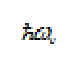
\includegraphics [scale=1] {image408}
	\captionsetup{labelformat=empty}
	\caption{Рис. 1 Схема энергетических зон квантовой проволоки Bi в постоянном электрическом поле} 
	\label{img:fig_4_4_1} 
\end{figure}

  
В дальнейшем для нанопроволок Bi рассмотрим простейшую модель перекрывающихся зон (рис. 1). На рис. 1. сплошными линиями изображены  размерно-квантованные уровни c и v зон. Пунктирными линиями представлены энергии носителей в постоянном электрическом поле.

Расчет термоэдс $\alpha _{xx} $ (слабое тянущее электрическое поле направленно вдоль оси x) проводился с использованием общих соотношений, связывающих $\alpha _{xx} $ с плотностью потока тепловой энергии $\gamma _{xx} $ для носителей и с электропроводностью для электронов и дырок \cite{Kubo1957}. В приближении времени релаксации \cite{Khamidullin2002} электропроводность и плотность потока тепловой энергии для электронов принимают вид:
\begin{equation} \label{eq:44_30}
\sigma _{xx}^{(c)} =\frac{\beta e^{2} \hbar ^{2} }{2Vm_{c}^{2} } \sum _{\alpha }k_{x}^{2} \tau _{\alpha }^{(c)} n_{\alpha } \left(1-n_{\alpha } \right) , (3a)
\end{equation}
\begin{equation} \label{eq:44_31}
\gamma _{xx}^{(c)} =\frac{\beta e^{2} \hbar ^{2} }{2Vm_{c}^{2} } \sum _{\alpha }\left(E_{\alpha }^{c} -\xi \right)k_{x}^{2} \tau _{\alpha }^{(c)} n_{\alpha } \left(1-n_{\alpha } \right) , (3b)
\end{equation}
\noindent здесь $n_{\alpha } $ -- равновесная функция распределения носителей с энергией $E_{\alpha }^{c} $, $\alpha $ -- набор квантовых чисел, описывающих состояние электрона, ${1 \mathord{\left/{\vphantom{1 \tau _{\alpha }^{(e)} }}\right.\kern-\nulldelimiterspace} \tau _{\alpha }^{(e)} } $ -- определяет полную квантово-механическую вероятность рассеяния частицы в единицу времени, $\xi $ -- химический потенциал исследуемой системы, $\beta ={1 \mathord{\left/{\vphantom{1 k_{0} T}}\right.\kern-\nulldelimiterspace} k_{0} T} $, T -- температура, V -- объем основной области наноструктуры.
 
Аналогично можно записать $\sigma _{xx}^{(h)} $, $\gamma _{xx}^{(h)} $ для дырок в v зоне. Расчет времени релаксации $\tau _{\alpha } $ проведем с учетом рассеяния носителей на шероховатой поверхности аналогично \cite{Karapetyan2011}. В случае $\delta $-образной флуктуации поверхности нетрудно получить:
\begin{equation} \label{eq:44_40}
\frac{1}{\tau _{\alpha }^{(c)} } =\frac{2m_{c} \omega _{c}^{2} \gamma _{0} }{\hbar R^{2} \left|k_{x} \right|} \left[n+k+1+N_{c} \right]^{2} , N_{c} =\frac{2\Delta _{c} }{\hbar \omega _{c} } ,
\end{equation} 
$\gamma _{0} $ -- описывает высоту флуктуации. При расчете времени релаксации для случая гауссовой флуктуации \cite{Vurgaftman1999} при низких температурах (именно при низких температурах рассеяние носителей на шероховатой поверхности наиболее активно) ${1 \mathord{\left/{\vphantom{1 \tau _{\alpha }^{(e)} }}\right.\kern-\nulldelimiterspace} \tau _{\alpha }^{(e)} } $ описывается соотношением (4), в котором нужно $\gamma _{0} $ заменить на $\pi \Delta _{0}^{2} \Lambda ^{2} $ ($\Delta _{0} $ -- высота гауссовой флуктуации, $\Lambda $ -- ее длина). Аналогично записывается $\tau _{\alpha }^{(h)} $ для дырок. В результате выражение для термоэдс после суммирования по $k_{x} $ принимает вид:
 
\begin{multline} \label{eq:44_50}
\alpha _{xx} =-\frac{k_{0} }{e} \left\{\sum _{n,m}\left[\nu \frac{F_{2} \left(\eta _{nm}^{c} \right)-\eta _{nm}^{c} F_{1} \left(\eta _{nm}^{c} \right)}{\left(n+m+1+N_{c} \right)^{2} } -\frac{F_{2} \left(\eta _{nm}^{v} \right)-\eta _{nm}^{v} F_{1} \left(\eta _{nm}^{v} \right)}{b\left(n+m+1+aN_{c} \right)^{2} } \right] \right\}\times\\
\times \left\{\sum _{n,m}\left[\nu \frac{F_{1} \left(\eta _{nm}^{c} \right)}{\left(n+m+1+N_{c} \right)^{2} } +\frac{F_{1} \left(\eta _{nm}^{v} \right)}{b\left(n+m+1+aN_{c} \right)^{2} } \right] \right\}^{-1}
\end{multline}
\[
a=\left(\frac{m_{h} }{m_{c} } \right)^{\frac{1}{2} } \left(\frac{\Delta E_{c} }{\Delta E_{h} } \right)^{\frac{3}{2} } , b=\frac{\Delta E_{h} }{\Delta E_{c} } ,
\] 
\[
\eta _{nm}^{c} =\beta \left[\Delta _{c} +\xi -\hbar \omega _{c} \left(n+m+1\right)\right],
\] 
\[
\eta _{nm}^{v} =\beta \left[\Delta +\Delta _{v} -\xi -\hbar \omega _{v} \left(n+m+1\right)\right],
\] 
\[
F_{k} (\eta )=\int _{0}^{\infty }dx \cdot x^{k} \cdot \frac{e^{x-\eta } }{\left(e^{x-\eta } +1\right)^{2} } , F_{1} (\eta )=\ln \left(e^{\eta } +1\right)
\] 
v -- количество зон проводимости, участвующих в кинетических процессах. Химический потенциал $\xi $ определяется из условия электронейтральности исследуемой наноструктуры (число электронов в размерно-квантованных c зонах равно числу дырок в v зоне):
\begin{equation} \label{eq:44_60}
\nu \sqrt{\frac{m_{c} }{m_{v} } } \sum _{n,m}F_{{\raise0.7ex\hbox{$ 1 $}\!\mathord{\left/{\vphantom{1 2}}\right.\kern-\nulldelimiterspace}\!\lower0.7ex\hbox{$ 2 $}} } \left(\eta _{nm}^{c} \right) =\sum _{n,m}F_{{\raise0.7ex\hbox{$ 1 $}\!\mathord{\left/{\vphantom{1 2}}\right.\kern-\nulldelimiterspace}\!\lower0.7ex\hbox{$ 2 $}} } \left(\eta _{nm}^{v} \right) .
\end{equation}
 
Аналитическое решение уравнения \eqref{eq:44_60} для химического потенциала можно найти для частных случаев.
 
Если носители находятся на нижайшем размерно-квантованном уровне ($n=m=0$), электронный и дырочный газ вырожден (химический потенциал положителен и $\beta \xi >>1$), то при $m_{c} <<m_{v} $, из \eqref{eq:44_60} не трудно определить $\xi $:
\[
\xi -\hbar \omega _{c} =\Delta +\Delta _{v} -\left(\hbar \omega _{c} +\hbar \omega _{v} \right), \left(\frac{\Delta _{v} }{\Delta _{c} } =\frac{\Delta E_{c} }{\Delta E_{v} } >1\right).
\] 
$\xi -\hbar \omega _{c} $ -- химический потенциал отсчитываемый от дна размерно-квантованной зоны.

В такой простой модели, термоэдс принимает вид:
\begin{equation} \label{eq:44_70}
\alpha _{xx} =-\frac{k_{0} }{e} \frac{\pi ^{3} }{3} \frac{1-\frac{1}{b\nu } \left(\frac{1+N_{c} }{1+aN_{c} } \right)^{2} }{\Delta +\Delta _{v} -\left(\hbar \omega _{c} +\hbar \omega _{v} \right)} .
\end{equation} 
Следовательно, термоэдс отрицательна, т.е. определяется электронами и с ростом напряженности электрического поля E уменьшается.

В противоположном случае невырожденного электронного и дырочного газов (это справедливо при малых радиусах квантовой проволоки $d<<500 \AA$Е, при $T=77 \text{ K}$ \cite{Black2002}), как следует из уравнения \eqref{eq:44_60}, химический потенциал определяется из соотношения:
\begin{equation} \label{eq:44_80}
\nu \sqrt{\frac{m_{c} }{m_{v} } } \exp \left(\eta _{00}^{c} \right)=\exp \left(\eta _{00}^{v} \right).
\end{equation}  
В результате
\begin{equation} \label{eq:44_90}
\alpha _{xx}^{(nd)} =-\frac{k_{0} }{e} \left\{2+\beta \left[\frac{1}{2} \ln (\nu ^{2} \frac{m_{c} }{m_{h} } )+\left(\hbar \omega _{c} +\hbar \omega _{v} -\Delta +\Delta _{v} +\Delta _{c} \right)\right]\right\},
\end{equation} 
 
Расчет термоэдс в общем случае проведен по соотношению \eqref{eq:44_50} с учетом размерно-квантованных v и c зон при типичных значениях параметров квантовой проволоки: $\Delta E_{c} =0.5 \text{ eV}$, $\Delta E_{v} =0.3 \text{ eV}$, $\Delta =0.038 \text{ eV}$, $m_{c} =0.01m_{0} $, $m_{v} =0.1m_{0} $, при $R=500 \AA$. Зависимость термоэдс от напряженности постоянного электрического поля приведена на рис. 2. 
 
\noindent \includegraphics*[width=6.16in, height=3.75in, keepaspectratio=false]{image414}
 
\noindent Рис. 2, Зависимость удельной термоэдс квантовой проволоки от напряженности поперечного электрического поля.
 
Кривая 1 получена при $T=10 \text{ K}$, кривая 2 вычислена при $T=50 \text{ K}$. Как показано на рис. 2. с ростом температуры величина термоэдс по абсолютной величине уменьшается и при увеличении E, стремится к нулю оставаясь при этом отрицательной.
 
В нанопроволоках, как следствие одномерности наноструктуры в плотности состояний на дне каждой размерно-квантованной зоны возникают особенности. Поэтому с ростом напряженности постоянного электрического поля экстремумы, например, размерно-квантованных v зон, поднимаясь вверх по энергии, могут пересекать химический потенциал, что, естественно, приводит к особенностям кинетических коэффициентов (например, подвижности). Однако в термоэдс эти особенности не очень ярко проявляются, поскольку $\alpha _{xx} $ определяется отношением потока тепловой энергии носителей к электропроводности.
 
При $E=0$ дырки вносят заметный вклад в термоэдс, уменьшая ее по абсолютной величине. С ростом напряженности электрического поля (для рассмотренных выше параметров нанопроволоки $a\sim 7$) вклад дырок в термоэдс быстро уменьшается, а это и приводит к тому, что в зависимости $\alpha _{xx} $ от $N_{c} $ (рис. 2) возникает характерный минимум.
 
Следовательно, внешнее электрическое поле дает уникальную возможность управлять величиной термоэдс, что позволяет надеяться  на приборное применение предсказанного эффекта. В заключение отметим, что сильная анизотропия эффективных эффективных масс в нанопроволоках Bi(в зависимости от направления кристаллографических осей массы для электронов в С-зоне меняются от $0,001m_{0} $ до $0,26m_{0} $, валентной зоне от $0,059m_{0} $ до $0,634m_{0} $ \cite{Levin2009a}) влияет на величину рассматриваемого эффекта, что сохраняет зависимость термоэдс от E практически неизменной.
